\chapter{Privacy Protection}

The goal of this document to analyze and identify the threads to personal privacy that are posed by collecting, storing and processing sensor data from mobile phones.
We derive concrete privacy protection measures that address the main risks involved with handling such data.
In the last part we describe how these measures are implemented in the Live+Gov toolkit.

As privacy is a very general and hard to grasp term, we need to fix a definition of privacy that is suitable for our needs.
As background information we include an overview about historical treatments of privacy as well as legal regulation of privacy in the European Union.
Based on this we propose a definition of privacy as {\em control over personal data}, and introduce a taxonomy of privacy attributes that give specify the term {\em personal data} in the context of mobile
sensor data collection.

The complexity of our systems and the variety of threads make a great number of counter measures plausible.
We approach this complexity with the aid of a general security analysis model developed in [Grimm].
We give a brief introduction to this model and perform a IT Security Analysis with respect to the privacy asset for our system.

\section{Histrocial Approaches to Privacy}

\subsection{Aristotle}

Public Sphere vs. Private Sphere of politics. This distinction is concerned with the politic (public) life of politicians in early democracies opposed by their domestic (private) life.

\subsection{Warren and Brandeis}

The Right to Privacy, 1890: Establish the term Informational Privacy. They argue innovations like photography and a growing press create the need for a new right to privacy, "the right to be left alone".

The term informational privacy as conceptual foundation of privacy originates from the juristic discussion The Right to Privacy (1890) by Warren and Brandeis.
The arise of new technologies like photography combined with a growing press created an increased publicity.
Warren and Brandeis were worried that existing law like castle doctrines or libel and slander could not suffice.
They felt a need for a new right to "protect the extent to wich one's thoughts, sentiments, and emotions could be shared with others" [1].
This right would be "the right to be left alone".

The right to "protect the extent to wich one's thoughts, sentiments, and emotions could be shared with others" by Warren and Brandeis was later extend to cover arbitrary information and is now kown as the privacy concept "... the control we have over information about ourselves ..." [2].

\subsection{Fried}

C. Freid, An Anatomy of Values, Harvard Univ. Press, 1970

Defines privacy as the ability to control information about oneself. He argues that limited knowledge does not automatically create privacy.

\section{Legal Aspects of Privacy}

* Present legal view on privacy from European angle: ``Data Protection Directive`` and Implementation.

* Some US Law

\subsection{European Convention on Human Rights - Article 8}

``(1) Everyone has the right to respect for his private and family life, his home and his correspondence. (2) There shall be no interference by a public authority with the exercise of this right except such as is in accordance with the law and is necessary in a democratic society in the interests of national security, public safety or the economic well-being of the country, for the prevention of disorder or crime, for the protection of health or morals, or for the protection of the rights and freedoms of others.'' {[}\hyperref[references]{3}{]}

``The European Court of Human has given this article a very broad
interpretation in its juresprudence.'' {[}\hyperref[references]{2}{]}

\subsection{EU Data Protection Direvtive}

\emph{Directive 95/46/EC}

EU directives in general do not hold any direct legal binding for EU citzens.
Member states have to create their own legal implementation.

``The directive regulates the processing of personal data regardless of whether such processing is automated or not.''
{[}\hyperref[references]{1}{]} where:

\begin{itemize}
\item
  \textbf{personal data} is ``any information relating to an identified or identifiable natural person {[}\ldots{}{]} (art. 2a)''
  {[}\hyperref[references]{1}{]}
\item
  \textbf{processing} is ``any operation or set of operations which is performed upon personal data {[}\ldots{}{]} (art. 2b)''
  {[}\hyperref[references]{1}{]}
\end{itemize}

The ``identified or identifiable natural person'' is called \textbf{data subject}.

The sole responsibility for compliance is held by so called \textbf{controllers}.
A controller is an actor ``which alone or jointly with others dertimines the purposes and means of the processing of personal data; (art 2d)''
{[}\hyperref[references]{1}{]}

This rule is applicable ``whenever the controller uses equipment situated within the EU''{[}\hyperref[references]{1}{]}.
This will hold for every e-commerce provider \textbf{inside or outside} of the EU because the customer's computer is \emph{situated within the EU} anyways.

``Personal data should not be processed at all, except when certain conditions are met'' {[}\hyperref[references]{1}{]}.
These conditions incorporate the seven OECD princepals and are futher categorized in the categories:

\begin{itemize}
\item
\textbf{Transparency}: ``The data subject has the right to be informed when his personal data is being processed {[}\ldots{}{]} (art. 10 and 11)'' {[}\hyperref[references]{1}{]} and he has the right how and by whom it is processed.
Additionally other speficied requirements have to be met, i.e.~giving consent.
\item
\textbf{Legitimate prupose}: ``Personal data can only be processed for specified explicit and legitimate pruposes and may not be processes futher in a way incompatible with those pruposes (art. 6b)''
{[}\hyperref[references]{1}{]}.
\item
\textbf{Proportionality}: ``Personal data may be processed only insofar as it is adequate {[}\ldots{}{]} in relation to {[}its{]} pruposes {[}\ldots{}{]}; every reasonable step must be taken to ensure that data wich are inaccurate or incomplete {[}\ldots{}{]} are erased or rectified (art. 6)'' {[}\hyperref[references]{1}{]}
\end{itemize}

(\textbf{Note:} The principles incorporated by the EU directive seem to closely map to \emph{the seven principles for user privacy control}.)

Member states have to create independent \textbf{supervisory authorities} for personal data processing where controllers have to register before they start to process any data.
The record has to be stored in public register {[}\hyperref[references]{1}{]}.

Data transfer to thrid countries outside of the EU requires those countries to have a similar data protection level. Exceptions exists:

\begin{itemize}
\item
  Save Harbor
\item
  Passenger Name Record Aggreement
\end{itemize}

all between the US and the EU, although the US has no comparable law of data protection. 
The US Supreme Court regards privacy as \textbf{implicit} right granted with the First Amendment. However, european law states privacy as \textbf{explicit} right (ECHR Art. 8).
Additionally the US government follows a doctrine which favors the economy to implement self-regulation {[}\hyperref[references]{1}{]}.

\subsection{Implementation of the Data Protection Direvtive}

\subsubsection*{Germany}

Germany implements Directive 95/46 with the \emph{Federal Data Protection Act} from 2001 known as \emph{Bundesdatenschutzgesetz (BDSG)} {[}\hyperref[references]{1}{]}{[}\hyperref[references]{2}{]}{[}\hyperref[references]{6}{]}.
However, Germany has violated the directive in two points:

\begin{enumerate}
\item
The BDSG has become effective three years too late, thus the EC filed a treaty violation proceeding against Germany {[}\hyperref[references]{6}{]}.

\item
The BDSG does not implement \textbf{independet} supervisory authorities. 
The \emph{Bundesdatenschutzbeauftragter} is subordinate to the Ministiry of Interior. 
Although he is not subject to technical oversight (\emph{Fachaufsicht}), he is subject to staff supervision by the government (\emph{Rechtsaufsicht} durch die Bundesregierung und  \emph{Dienstaufsicht} durch das Innenministerium) and budget oversight (including approval of employees) by the ministry {[}\hyperref[references]{7}{]}. 
Thus the EC filed a treaty violation proceeding against Germany, again {[}\hyperref[references]{6}{]}. 
In March 2010 Germany was found guilty of violation of Directive 95/46 by the ECJ {[}\hyperref[references]{6}{]}.
\end{enumerate}

Germany still violates point 2!

The states of Germany have their own implementation of Directive 95/46 (\emph{Landesdatenschutzgesetze}).
Federal public authorites are only bound to their federal law. {[}\hyperref[references]{2}{]}

Churches are not subject the BDSG. {[}\hyperref[references]{2}{]}

\begin{itemize}

\item
\textbf{Roman Catholic Church:}
\href{http://de.wikipedia.org/wiki/Anordnung_\%C3\%BCber_den_kirchlichen_Datenschutz}{Anordnung  über den kirchlichen Datenschutz (KDO)}

\item
\textbf{German Protestant Churches (Synode der Evangelischen Kirche in Deutschland):}
\href{http://de.wikipedia.org/wiki/Datenschutzgesetz_der_Evangelischen_Kirche_in_Deutschland}{Kirchengesetz  über den Datenschutz der Evangelischen Kirche in Deutschland}
\end{itemize}

Data subjects have the following rights.

\begin{itemize}
\item
Right to disclosure of wether data about them is stored and processed, which data is stored and processed and the data sources.
\item
Right to correction of false data.

\item
Right to file complaints to the supervisory authority.

\item
Right to have data deleted or blocked, but controllers can prohibit deletion in favour of blocking.

\item
Right to decline third party access to the data.
\end{itemize}

\subsubsection*{United Kingdom}

The UK implements Directive 95/46 with the \emph{Data Protection Act 1998 (DPA)} {[}\hyperref[references]{1}{]}{[}\hyperref[references]{3}{]}.

The act is knwon for its high complexity: a manual record of phone numbers for business purposes could be hold subject to the DPA {[}\hyperref[references]{3}{]}.
Although the act seems to fully cover the directive.
Even higher restriction apply for \emph{``sensitive personal data''} (race, ethnicity, politics, religion, trade union status, health, sex life or criminal record), i.e. \textbf{consent} must be given freely and has to be explicit. {[}\hyperref[references]{3}{]}

\emph{``The Act's definition of''personal data" covers any data that can be used to identify a living individual. Anonymised or aggregated data is not regulated by the Act, providing the anonymisation or aggregation has not been done in a reversible way.
Individuals can be identified by various means including their name and address, telephone number or
Email address.
The Act applies only to data which is held, or intended to be held, on computers (`equipment operating automatically in response to instructions given for that purpose'), or held in a `relevant filing system'.}

\emph{In some cases even a paper address book can be classified as a `relevant filing system', for example diaries used to support commercial activities such as a salesperson's diary.}

\emph{The Freedom of Information Act 2000 modified the act for public bodies and authorities, and the Durant case modified the interpretation of the act by providing case law and precedent.}

\emph{The Data Protection Act creates rights for those who have their data stored, and responsibilities for those who store, process or transmit such data.
The person who has their data processed has the right to:}

\begin{itemize}

\item
View the data an organisation holds on them.
A `subject access request' can be obtained for a nominal fee. As of January 2014, the maximum fee is £2 for requests to credit reference agencies, £50 for health and educational request, and £10 per individual otherwise.

\item
Request that incorrect information be corrected.
If the company ignores the request, a court can order the data to be corrected or destroyed, and in some cases compensation can be awarded.

\item
Require that data is not used in any way that may potentially cause damage or distress.

\item
Require that their data is not used for direct marketing. {[}\hyperref[references]{3}{]}
\end{itemize}

\subsubsection*{France}

France implements Directive 95/46 with Law 2004-801 modifying law 78-17 of 6.1.1978 (\emph{Loi n° 2004-801 du 6 août 2004} modifying \emph{loi n°78-17 relative à l'informatique, aux fichiers et aux libertés}) {[}\hyperref[references]{1}{]}{[}\hyperref[references]{10}{]}{[}\hyperref[references]{11}{]}.

\subsubsection*{United States of America}

The USA do not implement the directive, nor is there any obligation for them to do so.
However, companies subject to US jurisdiction can be certified to comply with the seven principles enforced by Directive 95/46 (the seven OECD recommendations) {[}\hyperref[references]{5}{]}.
Thus, those companies will act as \emph{safe harbors}. Without certification foreign companies are not allowed to send customer data back home {[}\hyperref[references]{9}{]}.

\emph{Safe harbor} in general is the legal concept to regulate that a certain conduct will be deemed {[}\hyperref[references]{4}{]}, but in germany the term is commonly used as synonym for the agreement between the EU and the US regarding Directive 95/46.)

\section{Privacy Definition and Taxonomy}

\subsection{Defining Privacy}

Defining privacy is a challenge which seems impossible. This is well put to words by Serge Gutwirth, who notes: \emph{``The notion of privacy remains out of the grasp of every academic chasing it. Even when it is cornered by such additional modifiers as `our' privacy, it still finds a way to remain elusive.''} {[}\hyperref[references]{2}{]}.

Many privacy researchers seem to ``forcus on the ways in which privacy can be infrenged'' {[}\hyperref[references]{1}{]}.
Thus they try to create taxonomies of \emph{privacy harms} instead of taxonomies of \emph{privacy types}.
Those two differ in the respect that the former focuses on threats to prohibit whereas the latter focuses on values to protect.
So one should rather evaluate what aspects are precious about privacy and develop measures to ensure their security than only forbid single actions against privacy {[}\hyperref[references]{1}{]}.

%% TODO %%

* We follow Fried in defining privacy as the ability to control data about personal information.

* What is the relation to legal aspects?

* What should be personal information?

* Use Seven Privacy Types be Friedewald, Finn and Wrigtht.

\subsection{The Seven Types of Privacy}

Seven Types of Privacy based on four types of privacy by Clarke.
Clarke's four types are outdated by contemporary technologies and no longer adequate. 
In order to fix this Friedewald, Finn and Wright extend the former four to the now introduced seven types privacy as follows:

\begin{enumerate}

\item \textbf{Privacy of the Person.}

This type is the right keep body functions and body characteristics
private {[}\hyperref[references]{1}{]}. It maps the one by Clarke.

Examples include:
\begin{itemize}
\item Body Characteristics: weight, height, sholder width, \ldots
\item Biometric Properties: Fingerprints, DNA Sequence, \ldots
\item Medical Conitions: Orthopedic conditions (e.g.~limping), Having a cold, \ldots
\end{itemize}

\item \textbf{Privacy of Behaviour and Action}

This type is also concerned with the ``protection against disclosure of personal matters'' {[}\hyperref[references]{1}{]} through behaviour, however Clarke's distinction between ``casual observation {[}\ldots{}{]} systematic recording and storage of information about those activities'' {[}\hyperref[references]{1}{]}is lifted.

Examples include:
\begin{itemize}
\item regular visit at church, backery, doctors
\item sexual habits
\item political activities
\end{itemize}

\item \textbf{Privacy of Communication}

It ``aims to avoid the interception of communications'' {[}\hyperref[references]{1}{]} either electronic or face-to-face.

Examples include:
\begin{itemize}
\item Secrecy of letters ('Briefgeheimnis' in german Legislation).
\item Email contents
\item Personal direct communication
\item Right to free discussion, i.e.~without third parties listening
\end{itemize}

\item \textbf{Privacy of Data and Image}

This type is concerned with ``making sure that individuals's data is not
automatically available to other individuals and organisations''
{[}\hyperref[references]{1}{]}. This is Informational Privacy in an
intuitive sense.

Examples include:
\begin{itemize}
\item Phone number
\item IP address
\item Public-administrative Data (Date of Birth, Melderegister)
\item Data held by organizations, like Banks or Insurance Companies
\item All data that is stored in online services (facebook)
\end{itemize}

\item \textbf{Privacy of Thoughts and Feelings}

This type is the right ``not to share their thoughts or feelings or to
have those thoughts or feeling (sic!) revealed''
{[}\hyperref[references]{1}{]}. It is concerned with (automatic) emotion
detection. This type is the counterpart the \emph{Privacy of the Person}
like body and mind are counterparts of one another (dualism).

Examples include:
\begin{itemize}
\item Current feeling: Depression, tiredness, stressed, awake
\item Thoughts in general.
\end{itemize}

\item \textbf{Privacy of Location and Space}

This type is the right ``to move about in public or semi-public space
withoug being identified, tracked or monitored'' {[}\hyperref[references]{1}{]}.
Additionally this type is concerned with the protection of one's home and private places (``right to solitude'' {[}\hyperref[references]{1}{]}).

Examples include:
\begin{itemize}
\item GPS position tracking
\item Location of home address
\end{itemize}

\item \textbf{Privacy of Association}

This type is the right ``to associate with whomever {[}one{]} wish, withoug being monitored'' {[}\hyperref[references]{1}{]}.
It is concerned with the protection against the automatic record of one's contacts.
It does not imply that one is monitored because of the associations.

Examples include:
\begin{itemize}
\item Friends
\item Joining of orgnaizations (e.g.~political parties)
\end{itemize}
\end{enumerate}

\subsection{Implicit Privacy Type Violation}

Cf. Figure \ref{figure:Implicit Privacy Violation Matrix}

%\includegraphics{../diagrams/png/implicit-privacy-violation-matrix.png}
\begin{figure}
\centering
\includegraphics[width=\textwidth]{diagrams/png/implicit-privacy-violation-matrix.png}

\begin{flushleft}
\scriptsize
\textbf{Legend:}
The matrix above shows the following relation: \emph{Type X can be
implicitly violated by the violation of type Y.}
\begin{itemize}
\itemsep1pt\parskip0pt\parsep0pt
\item
  The X-Axis shows the Seven Types of Privacy according to Friedewald et
  al., which could be violated implicitly
\item
  The Y-Axis shows the Seven Types of Privacy according to Friedewald et
  al., which have been violated explicitly
\item
  Big black bullet points denote, that an implicit violation is possible
\item
  Big grey bullet points only denote, that the relation is reflexive
  (\emph{a R a}). They are only shown for completeness sake and not
  discussed further, because they denote a trivial fact.
\end{itemize}
\end{flushleft}

\caption{Implicit Privacy Violation Matrix}
\label{figure:Implicit Privacy Violation Matrix}
\end{figure}

% =================================================
% Threat Table Macros

% Const Column Width
\newcommand{\ThreatTableColWidth}{5cm}

% Const Header Row Height
\newcommand{\ThreatTableHeaderRowHeight}{0.5cm}

% Const Content Row Height
\newcommand{\ThreatTableContentRowHeight}{1cm}

% Define Header Cell Makro
\newcommand{\ThreatTableHeaderCell}[1]{
\begin{minipage}[t][\ThreatTableHeaderRowHeight][c]{\ThreatTableColWidth}
\centering
\scriptsize
\textbf{#1}
\end{minipage}
}

% Define Content Cell Makro
\newcommand{\ThreatTableContentCell}[1]{
\begin{minipage}[t][][c]{\ThreatTableColWidth}
\begin{flushleft}
\tiny
#1
\newline
\end{flushleft}
\end{minipage}
}

% Define Header Row Makro
\newcommand{\ThreatTableHeaderRow}[4]{
\ThreatTableHeaderCell{#1}
&\ThreatTableHeaderCell{#2}
&\ThreatTableHeaderCell{#3}
&\ThreatTableHeaderCell{#4}
\\ \hline
}

% Define Content Row Makro
\newcommand{\ThreatTableContentRow}[4]{
\ThreatTableContentCell{#1}
&\ThreatTableContentCell{#2}
&\ThreatTableContentCell{#3}
&\ThreatTableContentCell{#4}
\\ \hline
}

%  Define Threat Table Environment
\newenvironment{ThreatTable}
{
\begin{tabular}{|c|c|c|c|}
\hline
\ThreatTableHeaderRow
{Description}
{Conflict of Interest}
{Vulnerabilites}
{Assets (Privacy Types)}
}
{\end{tabular}}


% =================================================
% Threat Table Content

\begin{landscape}
\begin{figure}
\centering
\begin{ThreatTable}

\ThreatTableContentRow
{\textbf{(Zero Day) Exploits}
\\A criminal uses (Zero Day) Exploits to obtain access to hardware or software which stores or processes
privacy sensitive data in order to get that data.}
{Criminals want to obtain access or data for personal profit, i.e. by (re-)selling the data or  by processing it themselves. 
However, criminals may have no financial interest, they could also gain personal (ego) profit by testing proof-of-concept attacks.
\\\textbf{Criminal vs Citizen}
\\Citizens only allowed Local Authorities to use their data. They want their data to be secret to others. (Additionally, citizens are
also interested in a working system, which they payed for via taxes.)
\\\textbf{Criminal vs Local Authorities}
\\Local Authorities have capital and reputation invested in a working system. Successful attacks undermine both.
\\\textbf{Criminal vs Maintenance Staff}
\\Staff members have a professional ethos and a duty to provide working systems. Successful attacks offend the former and obstruct the latter.
\\Staff member employed by L+G or contractor. The Business operation is thretened by loss of confidential data.
}
{Unsecured Hardware- or Software-Interfaces}
{\textbf{Explicit:} 1,4,6,7}

\ThreatTableContentRow
{\textbf{Man in the Middle} 
\\A criminal intercepts communication between mobile device and server or between server and application.}
{\textit{Like Exploits}}
{Unencrypted hardware or software communication}
{\textbf{Explicit:} 1,4,6,7}

\ThreatTableContentRow
{\textbf{Corrupt Employees} 
\\ An employee abuses his database access to obtain private citizen data in order to sell it to advertisers.}
{\textbf{(Corrupt) Employee vs Citizen} 
\\ Corrupt Employees want to make personal profit by selling citizen data. 
Citizens provide data for public improvement, they don't want their data to be used for other purposes, which
may lead to negative effects for themselves.
Employees in general need easy database access to do their job. But this also means easy access to privacy
sensitive data of citizens. This diametrically opposes the interest of citizens to have such information unknown
to other individuals.}
{Full database access of Employees}
{\textbf{Explicit:} 1,4,6,7}

\ThreatTableContentRow
{\textbf{Corrupt Local Authorities}
\\A member of the Local Authority abuses his access to applications 
to obtain aggregated citizen data in order to use it for illegitimate purposes, e.g. selling it.}
{\textbf{(Corrupt) Local Authority Member vs Citizen}
\\\textit{Like Corrupt Employees}}
{Full application access of Local Authorities}
{\textbf{Explicit:} 1,4,6,7}

\ThreatTableContentRow
{\textbf{Careless Citizen}
\\A careless citizen allows others (Criminals) to have unrestricted access to his mobile device. 
Hence, he creates to possibility to install spy-ware or have the device destroyed.}
{\textbf{Criminal vs Citizen}
\\Criminals want to have access to mobile devices to obtain private data of citizens in order to 
gain personal profit - or to simply render the device useless. On the other hand, citizens have a 
natural interest in keeping personal data secret in order to prevent financial loss or because having
sensitive information accessible to others violates their privacy.}
{Insufficient access rules for mobile devices}
{\textbf{Explicit:} 1,4,6,7}

\ThreatTableContentRow
{\textbf{Intransparent Data Mining}
\\Local Authorities or System Providers use their technical knowledge, data mining capabilities and 
additional data sources to obtain/create more information about citizens.}
{\textbf{Citizen vs Local Authority or System Provider}
\\Citizens only agreed to share certain sensitive data with Local Authorities and System Providers to help society.
They are not interested in negative effects as a result of such a good willing act.
However, Local Authorities and System Providers have an interest to maximize the profit of their investments.
Local Authorities could (secretly) use mined data for security or health care issues. System Providers could
(secretly) sell mined data to illegitimate customers, e.g. the SCHUFA. This could lead to repressive behaviour of law
enforcement or negative scores.}
{Unaware Citizens}
{1,2,3,4,5,6,7}

\end{ThreatTable}

{\scriptsize (\textbf{Note for Meeting:} I think we need discrete (numbered) lists of interests for each actor in the \textit{Humans} section.)}

\caption{Threat Table}
\end{figure}
\end{landscape}


\subparagraph{Privacy of The Person}

The Privacy of The Person is concerned with one's biometric privacy. If
this type is violated, following implicit violations are possible:

\begin{itemize}
\itemsep1pt\parskip0pt\parsep0pt
\item
  \textbf{Privacy of The Person:} reflexive violation
\item
  \textbf{Privacy of Behaviour and Action:} none
\item
  \textbf{Privacy of Communication:} none
\item
  \textbf{Privacy of Data and Image:} none
\item
  \textbf{Privacy of Thoughts and Feelings:} Some psychological diseases
  (e.g.~depression) have physiological impact. Such physiological
  patterns could be detected.
\item
  \textbf{Privacy of Location and Space:} none
\item
  \textbf{Privacy of Association:} none
\end{itemize}

\subparagraph{Privacy of Behaviour and Action}

The Privacy of Behaviour and Action is concerned with one's privacy
regarding social activities (religious, political, sexual, \ldots{}). If
this type is violated, following implicit violations are possible:

\begin{itemize}
\itemsep1pt\parskip0pt\parsep0pt
\item
  \textbf{Privacy of The Person:} Religious practices may include body
  modifications (e.g.~circumcision).
\item
  \textbf{Privacy of Behaviour and Action:} reflexive violation
\item
  \textbf{Privacy of Communication:} none
\item
  \textbf{Privacy of Data and Image:} none
\item
  \textbf{Privacy of Thoughts and Feelings:} Social activities in
  general depend on a certain intellectual attitude. Such an actvity is
  the expressions of such an attitude.
\item
  \textbf{Privacy of Location and Space:} none
\item
  \textbf{Privacy of Association:} Recording religious, politcal or
  sexual activities can reveal association with churches, political
  parties or sexual partners.
\end{itemize}

\subparagraph{Privacy of Communication}

The Privacy of Communication is concerned with not havin such
communication (corresponence or vis-a-vis) intercepted. This is very
broad type of privacy. Depending on the contens of the intercepted
communication every other type can be violated:

\begin{itemize}
\itemsep1pt\parskip0pt\parsep0pt
\item
  \textbf{Privacy of The Person:} Communication about body
  characteristics.
\item
  \textbf{Privacy of Behaviour and Action:} Communicatio about social
  activities.
\item
  \textbf{Privacy of Communication:} reflexive violation
\item
  \textbf{Privacy of Data and Image:} Communication containing one's
  passwords or other sensitive data.
\item
  \textbf{Privacy of Thoughts and Feelings:} Communication of thoughts
  and feelings, e.g.~wiretapping a flirt or a catholic confession
  ritual.
\item
  \textbf{Privacy of Location and Space:} Interception of face-to-face
  communication is only possible if one's location and space is violated
  (wiretapping).
\item
  \textbf{Privacy of Association:} Communication about one's
  associations (family members, churches, etc.).
\end{itemize}

\subparagraph{Privacy of Data and Image}

The Privacy of Data and Image is concered with one's data not beeing
automatically availabel to others. This also is a very broad type of
privacy. Depending of the data or image contents erery other type can be
violated:

\begin{itemize}
\itemsep1pt\parskip0pt\parsep0pt
\item
  \textbf{Privacy of The Person:} Images or stored biometric information
  reveal one's physical characteristics.
\item
  \textbf{Privacy of Behaviour and Action:} Images or diaries can reveal
  one's social activities.
\item
  \textbf{Privacy of Communication:} Modern communication systems
  usually contain some sort of archive function, e.g.~E-mail clients do
  not automatically delete messages. Such messages are data and reveal
  one's communication.
\item
  \textbf{Privacy of Data and Image:} reflexive violation
\item
  \textbf{Privacy of Thoughts and Feelings:} Images can show one's
  emotional state.
\item
  \textbf{Privacy of Location and Space:} Images can reveal one's
  location, e.g.~making a picture in front of the Eifel Tower.
\item
  \textbf{Privacy of Association:} E-mail data can also reveal
  association.
\end{itemize}

\subparagraph{Privacy of Thoughts and Feelings}

The Privacy of Thoughts and Feelings is concerned with keeping such
thoughts and feelings secret. If this type is violated, following
implicit violations are possible:

\begin{itemize}
\itemsep1pt\parskip0pt\parsep0pt
\item
  \textbf{Privacy of The Person:} Thoughts and feelings can reveal
  medical conditions.
\item
  \textbf{Privacy of Behaviour and Action:} Thoughts and feelings can
  reveal a certain attitudes which create a foundation for certain
  social activities.
\item
  \textbf{Privacy of Communication:} none
\item
  \textbf{Privacy of Data and Image:} none
\item
  \textbf{Privacy of Thoughts and Feelings:} reflexive violation
\item
  \textbf{Privacy of Location and Space:} none
\item
  \textbf{Privacy of Association:} Thoughts and feelings can reveal
  individual association, e.g amorous feelings for a certain person.
\end{itemize}

\subparagraph{Privacy of Location and Space}

The Privacy of Location and Space is concerned with one's right to move
freely without being tracked and one's right to private places. If this
type is violated, following implicit violations are possible:

\begin{itemize}
\itemsep1pt\parskip0pt\parsep0pt
\item
  \textbf{Privacy of The Person:} Frequently visited doctors can reveal
  certain medical conditions, if such doctors are known specialsts. In
  general it could imply ill-being.
\item
  \textbf{Privacy of Behaviour and Action:} Frequently visited places in
  general can reveal association and hence implies social activities.
\item
  \textbf{Privacy of Communication:} If one's location is knwon, it is
  possible to intercept (wiretap) one's communication. This also may
  violate the right to private spaces.
\item
  \textbf{Privacy of Data and Image:} If one's location is known, it is
  possible shoot pictures. This violates the right to one's image
  (\emph{``Recht am eigenen Bild''}).
\item
  \textbf{Privacy of Thoughts and Feelings:} Frequently visited persons
  may imply certain thoughts and feelings, e.g.~having a mistress.
\item
  \textbf{Privacy of Location and Space:} reflexive violation
\item
  \textbf{Privacy of Association:} Frequently visted places can reveal
  associations simply by searching in maps or yellow-pages.
\end{itemize}

\subparagraph{Privacy of Association}

The Privacy of Association is concerned with one's right to associate
with whomever one wants, without that association having recorded.If
this type is violated, following implicit violations are possible:

\begin{itemize}
\itemsep1pt\parskip0pt\parsep0pt
\item
  \textbf{Privacy of The Person:} Association with tatoo artists could
  imply having tatoos or other body modifications
\item
  \textbf{Privacy of Behaviour and Action:} Association with churches or
  poltical organizations could imply certain activities.
\item
  \textbf{Privacy of Communication:} none
\item
  \textbf{Privacy of Data and Image:} none
\item
  \textbf{Privacy of Thoughts and Feelings:} Association with churchs of
  political organizations could imply a certain intellectual attitude.
\item
  \textbf{Privacy of Location and Space:} none
\item
  \textbf{Privacy of Association:} reflexive violation
\end{itemize}



%%%%%%%%%%%%%%%%%%%%%%%%%%%%%%%%%%%%%%%%%%%%%%%%%%%%%%%%%%%%%%%%%%%%%
%%%%%%%%%%%%%%%%%%%%%%%%%%%%%%%%%%%%%%%%%%%%%%%%%%%%%%%%%%%%%%%%%%%%%
%%%%%%%%%%%%%%%%%%%%%%%%%%%%%%%%%%%%%%%%%%%%%%%%%%%%%%%%%%%%%%%%%%%%%

\section{IT Security}

\subsection{Basic Terminology}

%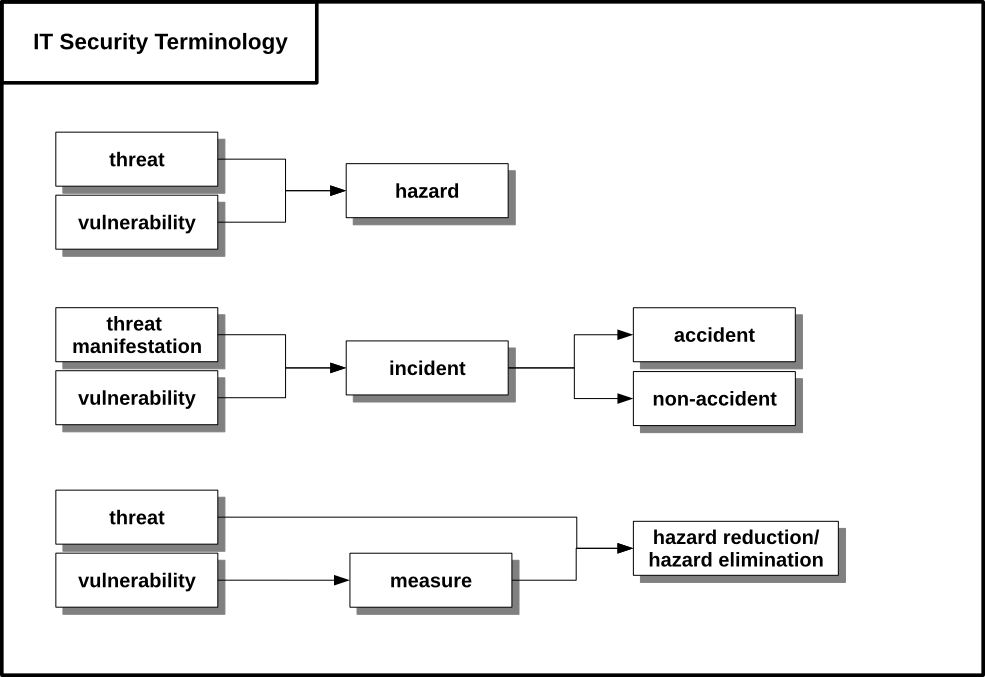
\includegraphics{diagrams/png/itsecterminology.png}
\begin{figure}
\centering
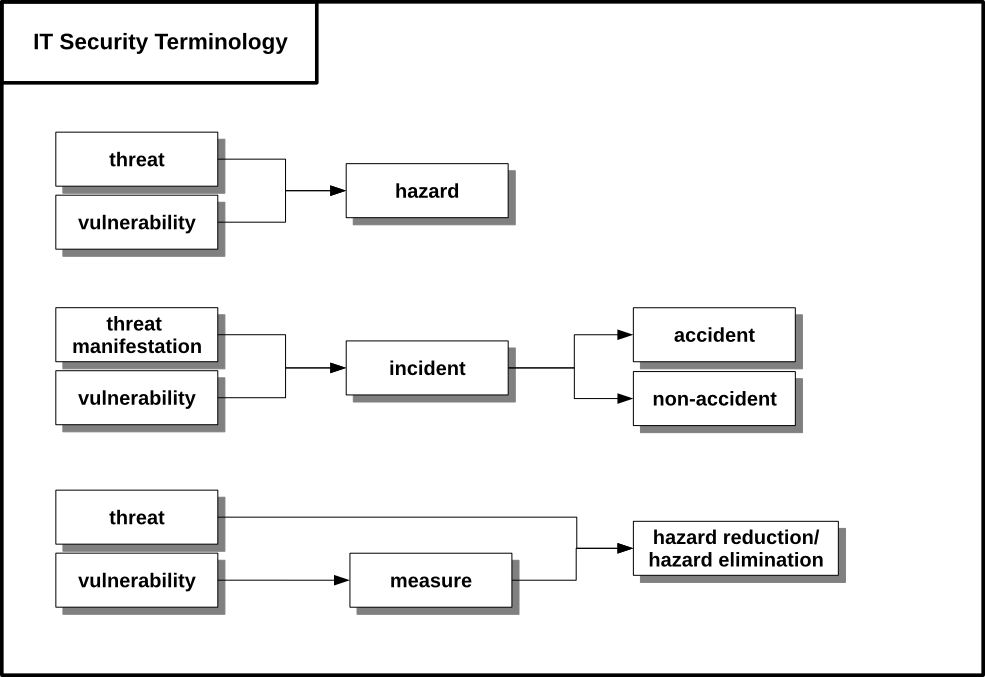
\includegraphics{diagrams/png/itsecterminology.png}
\caption{Basic IT Security Terminology}
\end{figure}


\subsubsection{threat}

\emph{threat} is a class of potential events whose manifestation can
cause damage or harm.

\subsubsection{vulnerability}

A weakness which can cause the loss of security.

\subsubsection{hazard}

Concrete risk due to one or more concrete vulnerabilities \textbf{AND}
corresponding threats.

\texttt{threat + vulnerability -\textgreater{} hazard}

\subsubsection{incident}

An event caused by a threat manifestation against one or more
corresponding vulnerabilities.

\texttt{threat manifestation + vulnerability -\textgreater{} hazard}

\subsubsection{accident}

An incident which did cause damage or harm. (Translates to
\emph{Schandensfall/Zwischenfall/Störfall} in german)

\subsubsection{non-accident}

An incident which \textbf{did not} cause any damage or harm.

\subsubsection{measure}

A well defined set of one or more activities which reduce or eliminate
vulnerabilities.

\subsection{IT Security Analysis according to Grimm et. al}

Grimm et al. create a reference model for conducting IT security
analyses consisting of:

\begin{itemize}
\itemsep1pt\parskip0pt\parsep0pt
\item
  an \textbf{ontology}, which aims to organize common security
  terminology in a reasonable and practical way
\item
  and a systematic analysis \textbf{procedure} based on that ontology
\end{itemize}

\subsubsection{Ontology}

%\includegraphics{../diagrams/png/itsec-ref-model-grimm.png}
\begin{figure}
\centering
\includegraphics[width=\textwidth]{diagrams/png/itsec-ref-model-grimm.png}
\caption{The IT Security Reference Model (Grimm)}
\end{figure}


\paragraph{Views}

The ontology is organized in four views:

\begin{itemize}
\itemsep1pt\parskip0pt\parsep0pt
\item
  \textbf{World:} Contains all components describing the current state.
\item
  \textbf{Potential:} Contains all components describing both the
  desired and dreaded state.
\item
  \textbf{Plan:} Contains all conceptual components required to develop
  sufficient measures to achieve and secure the desired state
  \textbf{or} to create the dreaded state. The \textbf{Plan} view
  \emph{realizes} the \textbf{Potential} view of the system.
  (\textbf{Note:} this should rather be translated with \emph{Concept})
\item
  \textbf{Event:} Contains all actual operations and events through out
  the production phase. The \textbf{Event} view \emph{instantiates} the
  \textbf{Plan} view of the system.
\end{itemize}

\paragraph{Components}

\subparagraph{World}

\begin{itemize}
\itemsep1pt\parskip0pt\parsep0pt
\item
  \textbf{Assets:} Things of value to one or more stakeholders. The
  value can be \emph{``hard''} (money, data, etc.) or \emph{``soft''}
  (trust,privacy,etc.).
\item
  \textbf{IT-Systems:} The IT-Systems under study.
\item
  \textbf{Humans:} All identifiable actors of the system under study.
  Many problems arise due to misunderstandings during man-machine
  interaction.
\item
  \textbf{Conflicts of Interests:} Different actors have different
  interests. Those interest can be in conflict. A trival conflict is the
  \emph{Attacker-Attackee}-Conflict: a service provider offers private
  data storage, therefore the provider is interested in having the
  access restricted. An attacker is naturally interested in easy access
  in order captialize the stolen data. However, heavy security
  restriction are also a burden for maintenance staff, as they are
  interested in having an easy life. This kind of conflict can create
  vulnerabilities.
\item
  \textbf{Vulnerabilities:} All indentifiable weaknesses in the current
  system layout.
\item
  \textbf{Interactions:} Assets, IT-Systems, Humans and Vulnerabilites
  are in continous interaction with each other in order to
  \emph{support} the \textbf{Business Objectives}. Those interactionscan
  also \emph{lead to} \textbf{Threats}, i.e.~having unencrypted
  communication with a server. Therefore all interactions which occur in
  the system's outline have to be documented.
\end{itemize}

\subparagraph{Potential}

\begin{itemize}
\itemsep1pt\parskip0pt\parsep0pt
\item
  \textbf{Chances/Risks:} Chances and Risks \emph{affect}
  \textbf{Business Objectives} (and \textbf{Threats}).
\item
  \textbf{Business Objectives:} Chances the system under study. This
  describes the desired state.
\item
  \textbf{Threats:} Risks for business objectives, this can simply be
  the integrety of the IT-System. Threats \emph{target} one or more
  \textbf{Assets} and violate \textbf{Security Requirements}. This
  describes the dreaded state.
\item
  \textbf{Security Requirements:} A set of distinct requirements for a
  safe and secure system. Security requirements \emph{hold for} one or
  more \textbf{Assets}. This describes the potential state after this
  procedure.
\end{itemize}

\subparagraph{Plan}

\begin{itemize}
\itemsep1pt\parskip0pt\parsep0pt
\item
  \textbf{Business Model:} The plan to achieve \textbf{Business
  Objectives}
\item
  \textbf{Accident Scenario:} This is either the plan of a certain
  attack or the concrete outline of random disaster. Although the latter
  is most likely hard to anticipate.
\item
  \textbf{Attack Technique:} A specific technique or technology to
  attack IT-Systems (Man in the Middel, Phishing, etc.). (\textbf{Note:}
  This component is not conform to the glossary as the term
  \emph{accident} there covers both disaster and attack!)
\item
  \textbf{Security Measures:} The plan to achieve a safe and secure
  system. Each \textbf{Security Mesaure} \emph{opposes} an
  \textbf{Accident Scenario} or an \textbf{Attack Technique}.
\end{itemize}

\subparagraph{Event}

\begin{itemize}
\itemsep1pt\parskip0pt\parsep0pt
\item
  \textbf{Business Process:} The actual, running instance of the
  \textbf{Busieness Modell}
\item
  \textbf{Accidents:} All actually happened accidents.
\item
  \textbf{Attacks:} All actually happened attacks. (\textbf{Note:} This
  component is not conform to the glossary as the term \emph{accident}
  there covers both disaster and attack!)
\item
  \textbf{Security Operations:} Instances of \textbf{Security Measures}.
  Security Measures \emph{secure} the system against \textbf{Accidents}
  and \textbf{Attacks}.
\end{itemize}

\subsubsection{Procedure}

The analysis procedure is an incremental and iterative process following
the four views of the previously described ontology.

%\includegraphics{../diagrams/png/itsec-ref-model-grimm-procedure.png}
\begin{figure}
\centering
\includegraphics{diagrams/png/itsec-ref-model-grimm-procedure.png}
\caption{The IT Security Reference Analysis (Grimm)}
\end{figure}


\paragraph{Step 1. World Analysis}

At first, one has to outline the current state of the system under
study. This includes description of:

\begin{itemize}
\itemsep1pt\parskip0pt\parsep0pt
\item
  all \textbf{Assets} which must be protected
\item
  all relevant \textbf{IT-Systems}
\item
  all involved \textbf{Humans} and their \textbf{Conflicts of Interests}
\item
  all known \textbf{Vulnerabilities}
\item
  and all important \textbf{Interactions} between the former components.
\end{itemize}

\paragraph{Step 2. Potential Analysis}

Secondly, one needs to outline the potential state of the system under
study. This includes both the dreaded (\textbf{Threats} and
\textbf{Risks}) and the desired (\textbf{Business Objectives},
\textbf{Chances}, \textbf{Security Requirements} state. This step
produces four artefacts:

\begin{itemize}
\itemsep1pt\parskip0pt\parsep0pt
\item
  a \emph{threat specifiation}, which identifies the \textbf{Threat} and
  its targeted \textbf{Assets}
\item
  a \emph{threat risk evaluation}, which detrmines the likelyhood of a
  threat manifestation
\item
  a \emph{hazard matrix}, which maps threats to known
  \textbf{Vulnerabilities} and identifies potential hazards
\item
  a \emph{security requirement specifiation}, which specifies
  requirments in order to deal with identified hazards
\end{itemize}

\paragraph{Step 3. Plan Development}

Based on \textbf{Step 2.}, the identified hazards are used alongside
realistic \textbf{Accident Scenarios} (\textbf{Attack Techniques}) to
create a \emph{risk matrix}. With this matrix it is possible to decide
if the risk is acceptable or not. Together with the previously specified
\textbf{Security Requirements}, the matrix is used to define adequate
\textbf{Security Measures}. Like a \textbf{Business Model} is an
abstract concept to achieve \textbf{Business Objectives}, this step
creates an abstract concept to improve the system's security.

\paragraph{Step 4. Plan Deployment}

Finally, the \textbf{Security Measures} have to be implemented.
Additionally, all \textbf{Business Operations}, \textbf{Accidents}
(\textbf{Attacks}) and executed \textbf{Security Operations} will be
recorded through out the production phase.

The implementation of \textbf{Security Measures} evantually changes the
\textbf{World} and renders the conducted analysis outdated. So this
analysis procedure needs to be conducted again.

\subsubsection{Abstraction Levels of the Reference Model}

The Reference Model can be used on different levels of abstraction. This
means each component can be used within a wide range of granularity, for
instance the security measure \emph{Encryption} can be explored in
genral or on the level of different concrete encryption tools; or on the
even finer level of concrete algorithms.

The utilized abstraction level is not important for the analysis
procedure, it depends on the intended audience for the analysis.
However, it is important to use one abstraction level consistently
through out the analysis.

\section{Live+Gov Privacy Protection Analysis}

\subsection{Step 1. World Analysis}

\subsubsection{Assets: Privacy}

We focus on the Asset privacy as described in Section \ref{sec:taxonomy}


\subsubsection{IT-Systems \& Humans}

\paragraph{Server Side Mining Scenario (Figure \ref{figure:Live+Gov Operation Scenario 01 - Server Side Mining})}

%\includegraphics{../diagrams/png/scenario01-ServerSideMining.png}
\begin{figure}[h]
\centering
\includegraphics{diagrams/png/scenario01-ServerSideMining.png}

\begin{flushleft}
\scriptsize
\textbf{Legend:}
\begin{itemize}
\itemsep1pt\parskip0pt\parsep0pt
\item
  \textbf{(a) Citizen:} User of the L+G client application whose privacy
  is at stake.
\item
  \textbf{(b) Mobile Device:} Runs the L+G client application, produces
  and stores data sensitive to the users privacy.
\item
  \textbf{(c) L+G Data Center:} Runs the L+G services, proccesses and
  stores user data.
\item
  \textbf{(d) L+G Maintenance Crew:} Technical staff with access to
  critical infrastructure.
\item
  \textbf{(e) Aggregation Monitor:} Interface to aggregated user data.
\item
  \textbf{(f) Local Authority:} Provider of the L+G system.
\end{itemize}
\end{flushleft}

\caption{Live+Gov Operation Scenario 01 - Server Side Mining}
\label{figure:Live+Gov Operation Scenario 01 - Server Side Mining}
\end{figure}



A citizen (a) carries a mobile device (b) running the L+G client. The
mobile device collects sensor data and sends it to the L+G Data Cetner
(c). The L+G Data Center also sends beneficial information for citizens
to the mobile device.

The L+G Maintenance Crew (d) maintaince the L+G Data Center.

The Aggregation Monitor (e) queries the L+G Data Center for aggregated
data. Local Authorities (f) use the Aggregation Monitor to get
information in order to improve public services. \textbf{In this
scenario the mobile the server conducts data mining on aggregated user
data and additionally trys to combine it with publicly accessible data
to enhance the results.}

When no connection to the L+G servers is available, the mining
end-products are stored on the mobile device.

\paragraph{Mobile Mining Scenario (Figure \ref{figure:Live+Gov Operation Scenario 02 - Mobile Mining})}

%\includegraphics{../diagrams/png/scenario02-MobileMining.png}
\begin{figure}
\centering
\includegraphics[width=\textwidth]{diagrams/png/scenario02-MobileMining.png}

\begin{flushleft}
\scriptsize
\textbf{Legend:}

\begin{itemize}
\itemsep1pt\parskip0pt\parsep0pt
\item
  \textbf{(a) Citizen:} User of the L+G client application whose privacy
  is at stake.
\item
  \textbf{(b) Mobile Device:} Runs the L+G client application, produces
  and stores data sensitive to the users privacy.
\item
  \textbf{(c) L+G Data Center:} Runs the L+G services, proccesses and
  stores user data.
\item
  \textbf{(d) L+G Maintenance Crew:} Technical staff with access to
  critical infrastructure.
\item
  \textbf{(e) Aggregation Monitor:} Interface to aggregated user data.
\item
  \textbf{(f) Local Authority:} Provider of the L+G system.
\end{itemize}
\end{flushleft}

\caption{Live+Gov Operation Scenario 02 - Mobile Mining}
\label{figure:Live+Gov Operation Scenario 02 - Mobile Mining}
\end{figure}


A citizen (a) carries a mobile device (b) running the L+G client. The
mobile device collects sensor data and sends it to the L+G Data Cetner
(c). The L+G Data Center also sends beneficial information for citizens
to the mobile device. \textbf{In this scenario the mobile device also
conducts data mining previously to sending the results to the L+G Data
Center.}

The L+G Maintenance Crew (d) maintaince the L+G Data Center.

The Aggregation Monitor (e) queries the L+G Data Center for aggregated
data. Local Authorities (f) use the Aggregation Monitor to get
information in order to improve public services.

When no connection to the L+G servers is available, the mining
end-products are stored on the mobile device.

\subsubsection{Conflict of Interests (Figure \ref{figure:Live+Gov Conflicts of Interests})}

%\includegraphics{../diagrams/png/conflict-of-interests.png}
\begin{figure}
\centering
\includegraphics[width=\textwidth]{diagrams/png/conflict-of-interests.png}
\caption{Live+Gov Conflicts of Interests}
\label{figure:Live+Gov Conflicts of Interests}
\end{figure}


\textbf{Citizen vs L+G Maintenance Crew}

\begin{itemize}
\itemsep1pt\parskip0pt\parsep0pt

\item Citizen want to exercise their legal right to privacy. I.e. their right to control information about themselves.
- citizens want to be unidentifiable
- citizens want certain informations about them to be secret
\item Citizen wants to prevent abuse of their private data, and the related negative consequences.
\item
  technical staff needs more or less unrestricted access to data in
  order to maintain the system
\end{itemize}

\textbf{Citizen vs Local Authority}

\begin{itemize}
\itemsep1pt\parskip0pt\parsep0pt
\item
  citizens want to be unidentifiable
\item
  citizens want certain informations about them to be secret
\end{itemize}

\textbf{L+G Maintenance Crew vs Local Authority}

\begin{itemize}
\itemsep1pt\parskip0pt\parsep0pt
\item
  staff wants proper payment
\item
  local authorities want to reduce cost
\end{itemize}

\textbf{Criminal vs Citizen}

\begin{itemize}
\itemsep1pt\parskip0pt\parsep0pt
\item
  citizens want to be unidentifiable
\item
  citizens want certain informations about them to be secret
\item
  criminals want to posses certain information about a citizen
\end{itemize}

\textbf{Criminal vs L+G Maintenance Crew}

\begin{itemize}
\itemsep1pt\parskip0pt\parsep0pt
\item
  criminals want to harm the system
\item
  technical staff has to keep the system safe and sound
\end{itemize}

\textbf{Criminal vs Local Authority}

\begin{itemize}
\itemsep1pt\parskip0pt\parsep0pt
\item
  criminals want to harm the system
\item
  criminals want access to collected data
\item
  local authorities have to keep collected data restricted
\item
  local authorities want a stable system
\end{itemize}

\subsubsection{Vulnerabilities}

%\includegraphics{../diagrams/png/scenario-vulnerabilities.png}
\begin{figure}
\centering
\includegraphics{diagrams/png/scenario-vulnerabilities.png}

\begin{flushleft}
\scriptsize
\textbf{Legend:}

\begin{itemize}
\itemsep1pt\parskip0pt\parsep0pt
\item
  \textbf{(a) Citizen:} User of the L+G client application whose privacy
  is at stake.
\item
  \textbf{(b) Mobile Device:} Runs the L+G client application, produces
  and stores data sensitive to the users privacy.
\item
  \textbf{(c) L+G Data Center:} Runs the L+G services, proccesses and
  stores user data.
\item
  \textbf{(d) L+G Maintenance Crew:} Technical staff with access to
  critical infrastructure.
\item
  \textbf{(e) Aggregation Monitor:} Interface to aggregated user data.
\item
  \textbf{(f) Local Authority:} Provider of the L+G system.
\item
  \textbf{(g) Criminal:} Threatens the L+G system and Citizen privacy.
\end{itemize}
\end{flushleft}

\caption{Live+Gov Vulnerabilities}
\label{figure:Live+Gov Vulnerabilities}
\end{figure}


\paragraph{Combined Scenario (Figure \ref{figure:Live+Gov Vulnerabilities})}

A citizen (a) carries a mobile device (b) running the L+G client. The
mobile device collects sensor data and sends it to the L+G Data Cetner
(c). The L+G Data Center also sends beneficial information for citizens
to the mobile device.

The L+G Maintenance Crew (d) maintaince the L+G Data Center.

The Aggregation Monitor (e) queries the L+G Data Center for aggregated
data. Local Authorities (f) use the Aggregation Monitor to get
information in order to improve public services.

A criminal (g) threatens the L+G system by corrupting the L+G
Maintenance Crew or Local Authority, or by forcing access to L+G
system's hardware, software or communication. (It is also possible for
criminals to corrupt the citizen, although technically this would be no
threat to privacy but rather an exercise of privacy
{[}\hyperref[references]{1}{]}.)

\paragraph{List of Vulnerabilities}

The vulnerabilities of Live+Gov system outline are:

\begin{itemize}
\item
  unencrypted data transmission (Man In The Middel)
\item
  insecure mobile devices (Exploit)
\item
  insecure servers (Exploit)
\item
  inadequate access rules for
  \begin{itemize}
  \item
    mobile devices (citizens)
  \item
    servers (staff)
  \item
    applications (local authority)
  \end{itemize}
\item
  corrupt/unhappy authorities or staff (\textbf{Could be actually a
  threat not a vulnerability})
\end{itemize}

(\textbf{Note:} The vulnerabilities seem to mostly open possibilities to
violate the \textbf{Privacy of Data and Image}, as this type is concerd
with making data \emph{automatically} available to others.)

\subsection{Step 2. Potential Analysis}

\subsubsection{Threats}

\begin{itemize}
\itemsep1pt\parskip0pt\parsep0pt
\item
  \textbf{Unauthorized access to privacy sensitive data}, caused by
  \begin{itemize}
  \item
    \textbf{Excessive Data Mining} Linking sensor data provided by
    citizens with additional sources can produce more privacy sensitive
    data.
  \item
    \textbf{Corrupt Local Authorities} Local Authorities have certain data
    access, they could hand over this access for monetary reasons.
  \item
    \textbf{Corrupt/Unhappy Staff} Staff members also have a certain data
    access and they also could hand over this access for monetary reasons
    or as a form of payback for unfair treatment.
  \item
    \textbf{Competent Attackers} Competent Attackers are always a threat
    for IT-systems. Normaly they have monetary reasons to exploit a
    system, but there is also a possibility for proof-of-concept like
    attacks.
  \end{itemize}
\end{itemize}


\paragraph{Sensor Privacy Matrix (Figure \ref{figure:Live+Gov Sensor-Privacy Matrix})}

%\includegraphics{../diagrams/png/sensor-privacy-matrix.png}
\begin{figure}
\centering
\includegraphics[width=\textwidth]{diagrams/png/sensor-privacy-matrix.png}


\begin{flushleft}
\scriptsize
\textbf{Legend:}
\begin{itemize}
\itemsep1pt\parskip0pt\parsep0pt
\item
  The x-axis lists the 7 Types of Privacy according to Friedewald et al.
\item
  The y-axis lists all mobile sensors currently used by the Live+Gov
  procject.
\item
  The big black bullet point dentotes that there is a \textbf{direct}
  violoation of a privacy type from a sensor
\end{itemize}
\end{flushleft}

\caption{Live+Gov Sensor-Privacy Matrix}
\label{figure:Live+Gov Sensor-Privacy Matrix}
\end{figure}




\subparagraph{Privacy of The Person}

The \textbf{Privacy of The Person} is generally concerned with one could
best understand as \emph{Biometric Privacy}. Friedewald et al. paraphase
it as \emph{``{[}\ldots{}{]} the right to keep body functions and body
characteristics {[}\ldots{}{]} private''}. \textbf{Accelerometer},
\textbf{Rotation Vector} and \textbf{Gyroscope} measure the physical
movement of the mobile device on all three axes. If the moblile device
is carried \emph{``normally''} its safe to say that those sensors also
measure the movments of its carrier. So his privacy is infringed
regarding biometric behaviour, as it is captured automatically.
(\textbf{Note:} This is not to be confused with the \textbf{Privacy of
Behaviour and Action} which is used for the social aspects of behaviour
action, e.g.~praying, sexual habits or poltical activities.)

\subparagraph{Privacy of Data and Image}

The \textbf{Privacy of Data and Image} demands, that
\emph{``individual's data is not automatically available to other
individuals''}. This type of privacy is trivially threatened because
here sensor data is indvidual data, a priori. So every sensor violates
the privacy of data and image, as data is transported into a foreign
system where operators have access to it.

\subparagraph{Privacy of Location and Space}

According to Friedewald et al., the \textbf{Privacy of Location and
Space} is concerned with one's \emph{``right to move about in public or
semi-public space withoug being identified, tracked or monitored.''}.
This is the location aspect of this type. The space aspect is concerned
with one's \emph{``right to solitude''}, which generally includes one's
right to an inviolate home and other private spaces. Obviously the
\textbf{GPS} and \textbf{GSM} sensors violate such right about not being
tracked, because they reveal the position of the mobile device and its
carrier. The \textbf{GSM} sensor gives the exact cell, the mobile device
has registered with at the current moment. The \textbf{GPS} sensor gives
the current longitude and latitude, the current global position of the
mobile device and its carrier, although there is some artificial
inaccuracy within civil use.

The \textbf{WLAN} and \textbf{Bluetooth} sensors record lists of the
currently available local wireless networks and bluetooth clients. If
such are known stationary entities, those sensors are considered as
dangerous as the \textbf{GSM} sensor for the carriers locational
privacy.

The \textbf{Magnetic field} sensor is not regarded very dangerous to the
carrier's privacy, because it does not allow very precise localization.
But it can limit the possibilities for the global position of the mobile
device. Here, it is just named for completeness sake.

\subparagraph{Privacy of Associtation}

The \textbf{Privacy of Association} sates that everyone has the
\emph{``right to associate with whomever they whish, without being
monitored {[}automatically without reasonable suspicion{]}''}. This
includes indivisuals and organizations. \textbf{WLAN} and
\textbf{Bluetooth} sensors provide the ability to monitor such
associations if their lists contain kown entities. If one frequently
connects with an organizational wirelss network, e.g.~an university
network, an association can be deduced (student or staff). The same goes
for the \textbf{Bluetooth} sensor, if it is stationary. Additionally, if
the recorded bluetooth clients are mobile, it is more or less possible
to deduce association with the technical identity of (yet) anonymous
individuals.

Additionally, the \textbf{GSM} sensor could provide the association with
the GSM operator (\textbf{NEEDS TO BE VERIFIED!}).

\paragraph{Excessive Data Mining}

\subparagraph{1 Privacy of the Person}

\emph{``This type is the right keep body functions and body
characteristics private''} {[}\hyperref[references]{1}{]}. Here we are
concerned with the personal physiological and psychological privacy of
citizens. This privacy is threatened if \textbf{body characteristics}
(weight, height, body measures, fingerprints, dna,\ldots{}) or
\textbf{medical conditions} (limping, having a cold, suffering from
depression, visiting therapists or other doctors) \textbf{can be
revealed or inferred}.

The Live+Gov project collects sensor data from mobile devices
(accellerometer, location, \ldots{}). By applying \emph{human activity
recognition (HAR)} techniques we could detect certain movement patterns
and in fact detect limping or other pathologic movements. Additionally
we know the position with of indiviual citizens with a sufficient
accurancy, and the Live+Gov project is only applied to a destinct urban
area. So we could link HAR data with the yellow pages, filter for
medical specialists and limit the possibilities of pathologic
conditions. But even without HAR data we could determine a likelihood
for certain conplaints. Frequent vistits to the dentist does not imply
healthy teeth.

\subparagraph{2 Privacy of Behaviour and Action}

\emph{``This type is also concerned with the `protection against
disclosure of personal matters' through behaviour''}
{[}\hyperref[references]{1}{]}. This type is concered with religous
practices, sexaul habits, political activities, etc. revealed through
observation. For the Live+Gove project this type is related to the
Privacy of Location and Space and the Privacy of Association. Locational
data is recorded by default and by linking it to maps and public
registers like phone books those *``personal matters*" could be
disclosed by frequently visited places (churches, brothels, party head
quaters, \ldots{}).

\subparagraph{3 Privacy of Communication}

\emph{``It `aims to avoid the interception of communications' either
electronic or face-to-face''} {[}\hyperref[references]{1}{]}. This type
is threatened if we intrude the secrecy of correspondence, posts and
telecommunications, personal direct communication or right to free
discussion without third parties listening. The Live+Giv project only
could threaten this type by using mobile client application as trojan
horse, collecting any communication data (chat, sms, microphone).

\subparagraph{4 Privacy of Data and Image}

\emph{``This type is concerned with `making sure that individuals's data
is not automatically available to other individuals and
organisations'\,''} {[}\hyperref[references]{1}{]}. This is
Informational Privacy in an intuitive sense regarding data like:

\begin{itemize}
\itemsep1pt\parskip0pt\parsep0pt
\item
  Phone Number
\item
  IP Address
\item
  Public-administrative Data (Date of Birth, population register)
\item
  Data held by organizations, like Banks or Insurance Companies
\item
  All data that is stored in online services (Facebook)
\end{itemize}

The Live+Gov project does not threaten this type directly if we assume a
secure and closed system. However, this privacy type could be threatened
by carelessly ignoring known (technical) vulnerabilities regarding data
security. Additionally we could threaten the Privacy of Data and Image
indirectly by linking collected data with other sources.

\subparagraph{5 Privacy of Thoughts and Feelings}

\emph{``This type is the right `not to share their thoughts or feelings
or to have those thoughts or feeling (sic!) revealed'\,''}
{[}\hyperref[references]{1}{]}. This means thoughts and emotions must
not be detected autmatically. Intuitively the Live+Gov system seems
unable to threaten this type. However, considering the issue component
of the Urban Maintaince use case, this might reveal information about
one's thoughts regarding the community in a positive manner. Solely by
taking part we could assume a caring personality. This threatens one's
privacy in a rather technical sense, but does not necessarily impose any
harm.

An other way of threatening this type could be constructed by recording
one's voice with the phone's microphone and run emotion detecting
algorithms against this data.

\subparagraph{6 Privacy of Location and Space}

\emph{``This type is the right `to move about in public or semi-public
space withoug being identified, tracked or monitored'. Additionally this
type is concerned with the protection of one's home and private places
(`right to solitude')''} {[}\hyperref[references]{1}{]}. The location
dimension of this type is relatively easy to understand: The
geo-position of citizens cannot be monitored by default. However, by
actively taking part in the Live+Gov project, the locational privacy of
citizens is threatened by default because data of the location sensor
will be collected. The space dimension is more complex, but can be
simplified with a \emph{``right to solitude''}. This dimension could be
threatend with the invasion of personal space in any means, i.e.~by
disrespecting one's right to an inviolate home or by undercutting one's
comfort zone in an conversation. Live+Gov only utilizes the mobile
devices of citizens, so we could disrespect the former by activating the
phone's micropone and start recording.

\subparagraph{7 Privacy of Association}

\emph{``This type is the right `to associate with whomever {[}one{]}
wish, withoug being monitored'.''} {[}\hyperref[references]{1}{]}. This
means that one's associations must not be recoreded by default
independet from any suspicion. Anyhow, it does not mean that this right
cannot be forfeit given a reasonable suspicion. The Live+Gov project
could easily threaten this type just by linking locational data with
yellow pages and a map. Even if an association graph cannot be deducted
for individual citizens, we could aggregate the data to create an
association graph for a whole population as the Live+Gov system is
applied to a restricted urban area.

\subsection{Step 3. Plan Development}

\subsubsection{Security Measures}

\paragraph{The 7 C's of user privacy control (Figure \ref{figure:The Seven Cs of User Privacy Control})}

This is a note on an excerpt from the article \emph{Sociotechnical
Architecture for Online Privacy} {[}\hyperref[references]{1}{]} called
\textbf{The 7 C's of user privacy control}. Those 7 C's are aspects
which should be covered by measures for implementing user privacy. They
derive from an interpretation of privacy which could be summarized as
\emph{``One's ability to control/seclude information about themselve''}.

%\includegraphics{../diagrams/png/The7Cs.png}
\begin{figure}
\centering
\includegraphics[width=\textwidth]{diagrams/png/The7Cs.png}
\caption{The Seven Cs of User Privacy Control}
\label{figure:The Seven Cs of User Privacy Control}
\end{figure}


\subparagraph{Comprehension}

\emph{``Users should \textbf{understand} ho personal identifiable
information (PII) is handled, who's collecting it and for what purpose,
and who will proccess the PII and for what purpose. Users are entitled
to know all parties that can access their PII, the limits to processing
transparency, why the PII data is being requested, when the data will
expire (Either from a collection or database), and what happens to it
after that. This category also include legal rights around PII, and the
imolications of a contract when one is formed.''}

This C implements transparancy regarding user data and user privacy.
Comprehension should answer the following questions:

\begin{itemize}
\itemsep1pt\parskip0pt\parsep0pt
\item
  \emph{WHO} collects data?
\item
  \emph{WHAT} data will be collected?
\item
  \emph{WHY} will data be collected and processed?
\item
  \emph{HOW} will data be collected and processed?
\item
  \emph{WHEN} will data expire?
\item
  What is allowed?
\item
  What choices ar possible?
\end{itemize}

All in all information of what's happening and why has to made
accessible for users.

\subparagraph{Consciousness \textbf{(critical!)}}

\emph{``Users should \textbf{be aware} of when data collections occurs,
when a contract is being formed between a user and data collector when
their PII is set to expire, who's collecting the data, with whom the
data will be shared, how to subsequently access the PII, and the
purposes for which the data is being collected.''}

This C seems to be critical for privacy protection. Consciousness
complements Comprehension in respect that the latter just states that
hard facts need to be delivered. However, those facts might get hidden
in a terms and conditions section which nobody reads but still accepts
anyway. In order to prevent that Consciousness states that a certain
level of \textbf{Awareness} of those facts needs to be establisched.

\subparagraph{Choice}

\emph{``Users should \textbf{have choices} regarding data collection
activies in terms of opting in or out, whether or not to provide data,
andhow to cerrect their data.''}

Self explaining. This is the actual control enabled by the 7 C's.

\subparagraph{Consnet}

\emph{``Users must first \textbf{consent} (meaning informed, explicit,
unambiguous agreement) to data collection, use, and storage proposals
for any PII. Privacy consent mechanisms should explicitly incorporate
the mechanisms of comprehension, consciousness, limitations, and
choice.''}

This C might be special case of Choice. Before taking part a user should
have the choice wether to join or not (Opt-In).

\subparagraph{Context}

\emph{``Users should \textbf{be able to change pricacy preferences}
according to context. Situational or physical context - such as crowded
situations (for example, when at a service desk where severeal people
can listen in on your exchange when you provide a phone number, or when
you're in an online community chat room) - is different from wehn you
perform a buy transaction with Amazon.com or in rooms with cameras
(where digitization makes the information permanent and unmistakably
you) and data context (such as the sensitivity of data, for example
health data could dictate different actions on the same PII in different
contexts.''}

Self explaining. Refines Choice in context sensitive manner.

\subparagraph{Confinement}

\emph{``Users should \textbf{be able to set limits} on who may access
their PII, for what purposes, and where and possibly when it may be
stored. Setting limits could provide some good opportiunities for future
negotiation between vendors and users.''}

Self explaining. Refines Choice regarding data collection and
processing.

\subparagraph{Consistency}

\emph{``Users should \textbf{anticipate} with reasonable certainty what
will occur if any action involving their PII is taken. That is, certain
actions should be predictable on user acces of PII or giving out of
PII.''}

Information given by Comprehension needs to be reliable to found
choices.

\paragraph{The 2 Steps of the 7 C's (Figure \ref{figure:The 2 Steps of the 7 Cs of User Privacy Control})}

If we look closer at the 7 C's and how they try to enable control, we
see that a 2 step approach is taken:

%\includegraphics{../diagrams/png/7Cs2Steps.png}
\begin{figure}
\centering
\includegraphics[width=\textwidth]{diagrams/png/7Cs2Steps.png}
\caption{The 2 Steps of the 7 Cs of User Privacy Control}
\label{figure:The 2 Steps of the 7 Cs of User Privacy Control}
\end{figure}


\subparagraph{(I) Enable \emph{Adequate} Control}

The 7 C's try to enable control through choices. A user should be able
to choose which data can be collected and processed depending on context
and who will have access to the data. But cannot be random. In order to
make substantiated choices and enable \emph{adequate} control a user
needs have

\begin{itemize}
\itemsep1pt\parskip0pt\parsep0pt
\item
  \textbf{Comprehension:} access to hard facts
\item
  \textbf{Consistency:} trust that those facts are reliable
\item
  \textbf{Conciousness:} awareness of those facts to found choices
\end{itemize}

\subparagraph{(II) Enable \emph{Actual} Control}

Naturally after creating a certain amount of knowledge, a user needs
also access to opportunities to make use of it. Therefore a user needs
possibilites to actually make choices. Additionally to having choices at
all, the 7 C's have 3 special choice categories:

\begin{itemize}
\itemsep1pt\parskip0pt\parsep0pt
\item
  \textbf{Choice}
  \begin{itemize}
  \item
    \textbf{Consent:} the choice to opt-in
  \item
    \textbf{Confinement:} the choice to set limits regarding user data
  \item
    \textbf{Context:} the choice to set limits regarding user data
    depending on certain context
  \end{itemize}

\end{itemize}

\section{References}
